\documentclass[conference]{IEEEtran}
\usepackage{cite}
\usepackage{amsmath,amssymb,amsfonts}
\usepackage{graphicx}
\usepackage{textcomp}
\usepackage{xcolor}
\usepackage{hyperref}
\usepackage{booktabs}
\usepackage{tabularx}
\usepackage{subcaption}

\hypersetup{
    colorlinks=true,
    linkcolor=blue,
    filecolor=magenta,      
    urlcolor=cyan,
    citecolor=blue,
}

\begin{document}

\title{A From-Scratch Swin Transformer vs.\ Pretrained CNN--LSTM: Architecture, Representation Health, and Benchmark on Radiology Image Captioning}

\author{
\IEEEauthorblockN{Naga Shiva\IEEEauthorrefmark{1}, Rajashree T\IEEEauthorrefmark{1}, Ravishanmugam\IEEEauthorrefmark{1}, Sharvesh Sivagnanam\IEEEauthorrefmark{1}}
\IEEEauthorblockA{\IEEEauthorrefmark{1}Department of Artificial Intelligence, Amrita School of Artificial Intelligence\\
Amrita Vishwa Vidyapeetham, Coimbatore, India\\}
}

\maketitle

\begin{abstract}
Medical image captioning aims to generate clear text descriptions from medical images, helping reduce reporting effort and improve consistency. In this work, we develop and evaluate an end-to-end framework for radiology image captioning on the ROCOv2 dataset, investigating two distinct architectural paradigms: (i) a hierarchical Vision Transformer encoder--decoder model implemented from first principles without pretrained backbones or third-party transformer libraries, and (ii) an established classical baseline pairing an ImageNet-pretrained ResNet-50 CNN encoder with a recurrent LSTM decoder. The Vision Transformer encoder is a Swin Transformer that converts a $224\times224$ image into hierarchical visual features using patch embedding, window-based self-attention, shifted-window attention, and patch merging. The final representation consists of 49 visual tokens, each with 768 dimensions, passed as memory to a six-layer Transformer decoder via cross-attention. An initial training run on ROCOv2 image--caption pairs exhibited severe encoder representation collapse: the 49 output tokens became nearly identical regardless of input content, and the decoder converged to a small set of generic, image-agnostic captions. We conduct a systematic audit to determine whether this failure originates in the architecture or the training recipe, first verifying architectural correctness with a mandatory ten-example overfitting test, then auditing the training code directly. The audit identifies three concrete recipe defects -- missing weight initialization, the absence of stochastic-depth regularization, and a learning-rate schedule that terminates just as training would otherwise recover -- which we fix and re-verify. Using the corrected recipe, we retrain the model at multiple data scales (2,000, 5,000, and the full 59,958 ROCOv2 training pairs) and re-run representation-health diagnostics. We further implement a pretrained ResNet-50 + LSTM baseline on the identical 9,927-image test split. We find that while the from-scratch Swin Transformer achieves spatial cross-attention across 49 tokens, transfer-learned pretraining combined with a two-phase training recipe elevates the Swin Transformer to surpass the CNN--LSTM baseline in sentence fluency (ROUGE-L: 0.2160 vs.\ 0.1953), clinical consensus (CIDEr-D: 0.3438), and caption diversity (79.8\% vs.\ 44.0\%), while matching it in higher-order precision (BLEU-4: 0.0379 vs.\ 0.0377). The CNN--LSTM retains faster inference throughput (5.75~ms vs.\ 45.2~ms). This comparative benchmark provides a fully transparent implementation, diagnostic methodology, and architectural analysis of vision-language modeling in radiology.
\end{abstract}

\begin{IEEEkeywords}
image captioning, Swin Transformer, transformer decoder, CNN--LSTM, ResNet-50, medical imaging, ROCOv2, vision-language models, attention mechanisms, representation collapse, inductive bias
\end{IEEEkeywords}

\section{Introduction}
\label{sec:intro}

Medical imaging generates a large volume of scans that must be interpreted and documented by trained radiologists. Preparing free-text descriptions is time-consuming and can introduce variation in how findings are described. Automatic medical image captioning aims to assist this process by generating natural-language descriptions directly from medical images, potentially providing a useful starting point for clinical documentation. However, medical image captioning is more challenging than captioning natural photographs because clinically relevant information can be subtle, spatially localized, and distributed across different regions of an image. A successful model must therefore capture both fine-grained visual patterns and the relationships between these patterns while producing coherent language.

Most image captioning systems follow an encoder--decoder architecture, in which a visual encoder converts an image into a feature representation and a language decoder generates a caption autoregressively. Convolutional neural networks have traditionally been used as visual encoders because of their strong ability to capture local spatial patterns. However, modeling long-range relationships with convolutional layers generally requires stacking multiple layers. Vision Transformers address this limitation by using self-attention to model relationships between image patches, but global self-attention becomes computationally expensive as the number of patches increases. The Swin Transformer addresses this problem by restricting self-attention to non-overlapping local windows and shifting the window partition between successive blocks. This design enables communication across neighboring windows while keeping the computational cost manageable. Its patch-merging operation further reduces spatial resolution and increases feature dimensionality, producing hierarchical visual representations at multiple scales.

In this work, we develop a radiology image captioning system that combines a Swin Transformer encoder with an autoregressive Transformer decoder. A central objective of the work is to understand and implement the complete architecture from first principles rather than relying on pretrained backbones or third-party Transformer implementations. The Swin encoder is constructed using elementary \texttt{torch.nn} operations and includes patch embedding, window partitioning and reversal, window-based multi-head self-attention (W-MSA), shifted-window multi-head self-attention (SW-MSA), learned relative position biases, attention masking, and patch merging. The encoder contains four hierarchical stages with depths $(2,2,6,2)$ and attention heads $(3,6,12,24)$, using a window size of $7$. Starting from a $224\times224\times3$ image, the encoder progressively produces a compact $7\times7\times768$ representation, corresponding to 49 visual tokens of dimension 768.

The resulting visual tokens are provided as memory to a six-layer Transformer decoder, which is also implemented from basic neural network operators. The decoder first represents caption tokens using a learned embedding and sinusoidal positional encoding. Each decoder layer then applies causally masked self-attention to model dependencies between previously available caption tokens, followed by cross-attention in which caption representations provide queries and the Swin visual tokens provide keys and values. This cross-attention mechanism forms the connection between the visual and language streams, allowing the decoder to use relevant image information while predicting each word. A position-wise feed-forward network then transforms the resulting representations.

An initial training run on the ROCOv2 dataset produced captions that were fluent but strikingly repetitive: a small number of generic, image-agnostic templates covered the large majority of generated outputs regardless of the input image. Rather than attribute this immediately to insufficient data or an under-parameterized decoder, we treat it as a diagnostic problem: is the failure architectural (a wiring, gradient-flow, or masking defect that would make the encoder incapable of learning regardless of data or recipe), or is it a training-recipe problem (correct architecture, poorly configured optimization)? We first isolate the architecture from the training recipe using a mandatory ten-example overfitting test -- if a correctly implemented model cannot memorize ten image--caption pairs, no amount of additional data or tuning will fix it. This test passes cleanly, ruling out an architectural defect and redirecting the investigation to the training code, where a direct audit identifies three concrete, fixable recipe defects. We apply the fixes, re-verify the overfitting test still passes, and then retrain at controlled data scales (2,000, 5,000, and full 59,958 images) to study how recipe correctness and data scale jointly affect representation health.

To provide a comprehensive benchmark against classical vision-language modeling, we additionally implement an ImageNet-pretrained CNN--LSTM baseline (ResNet-50 + linear projection + LSTM decoder) on the same dataset. We compare both models on the full 9,927-image test split across BLEU, ROUGE-L, METEOR, qualitative generation, and inference throughput.

The main contributions of this work are:
\begin{itemize}
    \item We implement a complete Swin Transformer encoder and autoregressive Transformer decoder from first principles for radiology image captioning, without pretrained model weights or third-party Transformer libraries.
    \item We provide a detailed implementation and analysis of the complete image-to-caption pipeline, including patch embedding, windowed and shifted-window attention, patch merging, caption self-attention, image--text cross-attention, and autoregressive word generation.
    \item We introduce a diagnostic methodology -- a mandatory small-batch overfitting test combined with a representation-health audit (within-image token similarity, variance decomposition, and a synthetic-image control experiment) -- that separates architectural defects from training-recipe defects, and use it to identify and fix three concrete recipe defects: missing weight initialization, absent stochastic-depth regularization, and an early-stopping/learning-rate schedule mismatch.
    \item We measure the effect of the corrected recipe combined with increasing training-data scale on representation collapse and caption quality, demonstrating an image-dependent reduction in collapse and monotonic improvement in caption diversity.
    \item We implement a classical pretrained ResNet-50 + LSTM baseline on the full ROCOv2 split, providing an empirical benchmark that contrasts from-scratch Vision Transformer dynamics with pretrained CNN inductive bias on identical test data.
\end{itemize}

The remainder of this paper is organized as follows. Section~\ref{sec:related} reviews related work in image captioning, vision Transformers, and medical report generation. Section~\ref{sec:method} describes the Swin encoder, Transformer decoder, training recipe corrections, and the CNN--LSTM baseline. Section~\ref{sec:experiments} presents the dataset, experimental setup, and evaluation protocol. Section~\ref{sec:results} reports the diagnostic findings, caption quality, and comparative benchmark. Finally, Section~\ref{sec:conclusion} summarizes conclusions and future scope.

\section{Related Work}
\label{sec:related}

\subsection{Classical and Attention-Based Image Captioning}
Early neural image captioning systems adopted an encoder--decoder design in which a convolutional neural network (CNN) encoder produced a single global image vector that was fed to a recurrent decoder. Vinyals et al.~\cite{vinyals2015show} introduced this paradigm with Show and Tell, pairing a CNN encoder with an LSTM decoder trained to maximize caption likelihood. Xu et al.~\cite{xu2015show} extended this with Show, Attend and Tell, adding a spatial attention mechanism so the decoder could focus on different CNN feature-map regions at each generation step, rather than relying on one compressed vector for the whole image. This attention-based CNN-LSTM design became the dominant template for captioning work over the following years and is the direct architectural ancestor of the CNN+LSTM system described by Pranay Kumar et al.~\cite{ijraset2022}, which trains a CNN feature extractor coupled with an LSTM decoder on the general-domain Flickr8k dataset. That work targets natural photographs (people, animals, everyday scenes) rather than medical images, and reports results at Flickr8k scale rather than on a radiology corpus; it is nonetheless a useful architectural reference point in this survey because it represents the CNN-LSTM baseline that Transformer-based encoder--decoder captioning, including the system in this paper, is intended to improve upon in modeling long-range dependencies between visual regions and generated words.

\subsection{Transformer Architectures and Vision Transformers}
Vaswani et al.~\cite{vaswani2017attention} proposed the Transformer, replacing recurrence with multi-head self-attention and showing that sequence modeling could be done more efficiently and with better long-range dependency capture than RNN/LSTM-based approaches. This architecture was originally developed for machine translation but its decoder block -- masked self-attention, cross-attention, and a position-wise feed-forward network -- is the same structure used by essentially all subsequent Transformer-based caption decoders, including the six-layer decoder used in this work. Dosovitskiy et al.~\cite{dosovitskiy2020vit} later showed with the Vision Transformer (ViT) that an image, split into fixed-size patches and treated as a token sequence, could be processed directly by a standard Transformer encoder without any convolutional inductive bias, provided sufficient pretraining data. However, ViT's global self-attention scales quadratically with the number of patches, which becomes expensive at high resolution. Liu et al.~\cite{liu2021swin} addressed this with the Swin Transformer, which restricts self-attention to non-overlapping local windows and alternates regular and shifted window partitions across successive blocks (W-MSA/SW-MSA) so that information can still propagate across window boundaries. Combined with a patch-merging operation that halves spatial resolution and doubles channel width between stages, Swin produces a hierarchical, multi-scale visual representation at linear rather than quadratic cost in the number of patches -- the property that motivates its use as the visual encoder in this work. Liu et al.\ also report stochastic-depth (DropPath) regularization as part of Swin's standard training recipe~\cite{liu2021swin}; its absence is one of the recipe defects we identify and correct in Section~\ref{sec:method}.

\subsection{Medical and Radiology Image Captioning}
Captioning in the medical domain is complicated by the fact that clinically relevant findings are often small, subtle, and spatially localized, and by the comparative scarcity of large, cleanly paired image--caption medical corpora relative to general-domain photography datasets. Pelka et al.~\cite{pelka2018roco} introduced ROCO (Radiology Objects in COntext), one of the first large-scale radiology image--caption datasets built from the PMC Open Access subset, enabling captioning research on real clinical figures rather than natural images. Rückert et al.~\cite{ruckert2024rocov2} released ROCOv2, an updated and expanded version of this dataset with improved image--caption--concept alignment, which is the dataset used for training and evaluation in this work (Section~\ref{sec:experiments}). ROCOv2 has since served as the basis for the ImageCLEFmedical Caption challenge; the 2023 edition's overview paper~\cite{ruckert2023imageclef} reports a DenseNet169-CNN-with-LSTM-decoder baseline against which the BLEU/ROUGE/CIDEr results in this paper are compared (Section~\ref{sec:results}). More recent work has moved from CNN-RNN pipelines toward Transformer-based medical captioning. Lee et al.~\cite{lee2022cross} propose a cross encoder--decoder Transformer with a global-local visual extractor for medical image captioning, combining coarse whole-image and fine region-level visual features before cross-attention decoding. Fadhilah and Utama~\cite{fadhilah2026transformer} similarly use a Transformer encoder--decoder for medical image captioning, augmented with UMLS concept-embedding supervision to ground generated text in clinical terminology. Both systems, like most recent medical captioning work, rely on CNN or pretrained Transformer backbones for the visual encoder; neither trains a Swin-style hierarchical window-attention encoder entirely from randomly initialized weights, which is the specific setting explored in this paper.

\subsection{Positioning of This Work}
Taken together, the literature above shows a clear architectural progression -- from CNN-LSTM encoder--decoder captioning~\cite{vinyals2015show,xu2015show,ijraset2022}, to attention-augmented CNN decoders, to fully Transformer-based encoder--decoder captioning built on ViT- or Swin-style visual backbones~\cite{dosovitskiy2020vit,liu2021swin,lee2022cross,fadhilah2026transformer} -- almost universally under the assumption of large-scale pretraining or at minimum a pretrained visual backbone. Medical captioning work built on ROCO/ROCOv2~\cite{pelka2018roco,ruckert2024rocov2,ruckert2023imageclef} typically follows the same pattern, pairing a pretrained CNN encoder (e.g., DenseNet169) with an LSTM or Transformer decoder. This paper instead studies a harder and less-explored setting: a Swin Transformer encoder and Transformer decoder implemented entirely from first principles and trained with randomly initialized weights, without any pretrained backbone, transformers library, or third-party captioning framework. Because a randomly initialized attention-based encoder has none of the inductive bias that ImageNet or masked-image pretraining would normally supply, it is also more exposed to the kind of representation collapse this paper investigates -- a failure mode in which the encoder's output becomes nearly image-independent and the decoder falls back to generic, high-frequency captions -- and to training-recipe sensitivities (initialization, regularization, learning-rate scheduling) that pretrained backbones are comparatively robust to. This framing positions the present work as a transparency- and diagnostics-focused complement to the pretrained-backbone medical captioning literature, alongside a direct benchmark comparison to a classical pretrained CNN--LSTM baseline.

\subsection{Literature Review Summary}
\label{sec:related-summary}

Table~\ref{tab:litreview} summarizes the eight papers most directly responsible for specific design decisions in this work, in the order they compose into the final system: the classical captioning paradigm and its attention mechanism~\cite{vinyals2015show,xu2015show}, the Transformer and vision-Transformer building blocks~\cite{vaswani2017attention,dosovitskiy2020vit,liu2021swin}, the dataset and benchmark this work is trained and measured against~\cite{ruckert2024rocov2,ruckert2023imageclef}, and the closest prior medical-domain Transformer captioning system~\cite{lee2022cross}.

\begin{table*}[t]
\centering
\caption{Literature review: core contribution of each paper, its methodology, and its specific role in this work's design.}
\label{tab:litreview}
\small
\begin{tabularx}{\textwidth}{@{}p{2.3cm}X X X@{}}
\toprule
\textbf{Paper} & \textbf{Core idea} & \textbf{Approach (what / how)} & \textbf{Role in this work} \\
\midrule

Vinyals et al., \emph{Show and Tell}~\cite{vinyals2015show} (2015)
&
Frame image captioning as end-to-end encoder--decoder learning, directly maximizing caption likelihood given an image -- borrowing the sequence-to-sequence framing from machine translation.
&
A CNN (Inception) pools the whole image into one global feature vector; an LSTM decoder is initialized from that vector and generates the caption word-by-word via teacher-forced cross-entropy training and beam search at inference.
&
Establishes the overall encoder$\to$decoder$\to$caption pipeline this work follows, but its single pooled vector is exactly the bottleneck we avoid in Swin: our encoder keeps 49 spatially distinct tokens instead of collapsing to one vector. \\

Xu et al., \emph{Show, Attend and Tell}~\cite{xu2015show} (2015)
&
Fix Show-and-Tell's bottleneck by keeping the CNN's full spatial feature grid and letting the decoder compute a soft attention distribution over it at every step.
&
CNN feature map (e.g.\ $14\times14$) retained as a set of location vectors; the LSTM decoder scores each location against its hidden state (additive attention), takes a weighted sum as context for the next word.
&
Direct conceptual ancestor of our cross-attention sub-layer: our decoder attends over the 49 Swin tokens exactly as theirs attends over CNN grid cells, reimplemented as Transformer scaled dot-product attention instead of additive LSTM attention. \\

Vaswani et al., \emph{Attention Is All You Need}~\cite{vaswani2017attention} (2017)
&
Replace recurrence entirely with multi-head self-attention, enabling full parallelism and stronger long-range modeling.
&
Encoder--decoder Transformer: multi-head scaled dot-product attention, causal self-attention masking, encoder--decoder cross-attention, sinusoidal positional encoding, residual+LayerNorm blocks, position-wise FFN, label smoothing.
&
The direct blueprint for our entire decoder (Section~III-B): our masked self-attention, cross-attention, sinusoidal positional encoding, and label-smoothed cross-entropy loss are this paper's recipe, reimplemented from primitive \texttt{torch.nn} layers. \\

Dosovitskiy et al., \emph{ViT}~\cite{dosovitskiy2020vit} (2020)
&
A pure Transformer, with no convolution, can do vision if an image is treated as a sequence of flattened patches.
&
Split image into fixed-size patches, linearly project each to an embedding (a conv with kernel=stride=patch\_size), add learned absolute position embeddings, feed through a standard global-attention Transformer encoder.
&
Source of our patch-embedding stage (Section~III-A.1) and its conv/linear-projection equivalence -- but we deliberately drop ViT's global attention and absolute position embeddings, since Swin (below) removes both. \\

Liu et al., \emph{Swin Transformer}~\cite{liu2021swin} (2021)
&
Fix ViT's quadratic attention cost and single-scale output by windowing attention and shifting the window grid between blocks, with periodic patch merging for a CNN-like feature pyramid.
&
4-stage hierarchical encoder; alternating W-MSA/SW-MSA blocks per stage; learned relative position bias per window instead of absolute encoding; PatchMerging halves resolution and doubles channels between stages; DropPath regularization across blocks.
&
This is the encoder we implemented block-for-block (Section~III-A), including the exact Swin-T depths/heads/window configuration. Critically, DropPath and Liu et al.'s weight-init scheme were the two pieces of their recipe we initially omitted -- and re-adding them, per Section~III-D, was a large part of fixing representation collapse in Section~V. \\

Rückert et al., \emph{ROCOv2}~\cite{ruckert2024rocov2} (2024)
&
Provide a large-scale, updated, better-curated radiology image--caption(--concept) dataset built from PubMed Central Open Access figures.
&
$\sim$80K radiology images (CT, MRI, X-ray, ultrasound, angiography, \ldots), each with a caption mined from its source figure legend, plus UMLS concept annotations per image.
&
The dataset this entire project trains and evaluates on (Section~IV-A). Every vocabulary size, split size, and result in Section~V is a direct consequence of this dataset's structure; its unused concept CSVs motivate the auxiliary-loss item in future work. \\

Rückert et al., \emph{ImageCLEFmedical 2023 Overview}~\cite{ruckert2023imageclef} (2023)
&
Define the shared-task benchmark for ROCOv2 caption generation and publish a reference baseline.
&
Pretrained DenseNet169 encoder $\to$ pooled feature $\to$ LSTM decoder, trained and scored on ROCOv2's official splits with BLEU/ROUGE/CIDEr-style metrics.
&
Our direct quantitative yardstick: every BLEU/ROUGE/CIDEr number we report is compared against this baseline, with the pretrained-vs.-random-init asymmetry explicitly flagged rather than treated as like-for-like. \\

Lee et al., \emph{Cross Encoder--Decoder Transformer}~\cite{lee2022cross} (2022)
&
Apply a Transformer encoder--decoder, rather than CNN-LSTM, to medical captioning, using a global-local visual extractor.
&
A pretrained backbone produces both a coarse whole-image descriptor and fine region-level descriptors; both are exposed to the decoder's cross-attention, letting each word draw on ``big picture'' or fine detail as needed.
&
Our closest architectural relative: our single Swin hierarchy yields coarse (Stage~4) and fine (Stage~1) features from one pyramid, substituting for their explicit dual-pathway extractor -- and unlike their pretrained backbone, ours is trained entirely from random initialization, which is this paper's central research question. \\

\bottomrule
\end{tabularx}
\end{table*}

\section{Methodology}
\label{sec:method}

\subsection{Swin Transformer Encoder}
\label{sec:method-encoder}

\subsubsection{Patch Embedding}
The input image is first divided into non-overlapping $4\times4$ patches using a stride-4 convolution (\texttt{PatchEmbed}), mathematically equivalent to flattening each patch and applying a shared linear projection. This produces a $56\times56$ grid of tokens with embedding dimension $C=96$, followed by layer normalization.

\subsubsection{Window and Shifted-Window Self-Attention}
Rather than computing self-attention across all $56\times56=3136$ tokens -- which would scale quadratically with token count -- the encoder partitions the token grid into non-overlapping $7\times7$ windows and restricts multi-head self-attention to within each window (\texttt{WindowAttention}). A learned relative position bias is added to the attention logits: for every possible relative offset $(\Delta h, \Delta w)$ between two positions inside a window, a bias term is looked up from a table of shape $(2\cdot7-1)^2 \times \text{heads}$ and added to the corresponding attention score, replacing the fixed absolute positional encoding used in the original Transformer.

Restricting attention to fixed windows would prevent tokens from ever exchanging information across window boundaries. Following the shifted-window design, alternating blocks within each stage cyclically shift the token grid by $\lfloor \text{window\_size}/2 \rfloor$ pixels before partitioning (\texttt{SwinBlock}, even-indexed blocks use regular W-MSA with \texttt{shift\_size=0}; odd-indexed blocks use shifted SW-MSA). Because the shift can create windows that mix content from non-adjacent regions of the original grid, an attention mask is precomputed per shifted block (\texttt{\_build\_shift\_mask}) that assigns a large negative bias ($-100.0$, rather than $-\infty$, to avoid a known softmax NaN issue on Apple MPS) to attention scores between tokens that were not spatially adjacent before the shift. Each block applies pre-norm residual connections around both the (shifted-)window attention and a two-layer GELU feed-forward MLP.

\subsubsection{Patch Merging and Hierarchical Stages}
After every stage except the last, a patch-merging layer (\texttt{PatchMerging}) concatenates each $2\times2$ neighborhood of tokens along the channel dimension, applies layer normalization, and linearly projects back down to $2C$ channels -- halving spatial resolution while doubling channel width. The encoder stacks four such stages (\texttt{BasicLayer}) with depths $(2,2,6,2)$ and attention head counts $(3,6,12,24)$, following the Swin-T configuration. Starting from $56\times56\times96$, the four stages progressively reduce the representation to $28\times28\times192 \rightarrow 14\times14\times384 \rightarrow 7\times7\times768$. A final layer normalization is applied, yielding $49$ visual tokens of dimension $768$, which serve as the memory input to the decoder.

\subsection{Transformer Decoder}
\label{sec:method-decoder}

The decoder (\texttt{CaptionDecoder}) is a six-layer autoregressive Transformer that generates the caption token by token, conditioned on the 49 Swin visual tokens.

\subsubsection{Token Embedding and Positional Encoding}
Caption tokens are mapped to $d_{model}=768$-dimensional vectors through a learned embedding table, matching the encoder's output dimension so no additional projection is needed between encoder and decoder. Fixed sinusoidal positional encodings (\texttt{PositionalEncoding}) are added to the token embeddings to inject sequence-order information.

\subsubsection{Decoder Layer: Masked Self-Attention, Cross-Attention, Feed-Forward}
Each of the six decoder layers (\texttt{DecoderLayer}) applies three sub-layers in sequence, each wrapped in a residual connection followed by post-layer-norm:
\begin{enumerate}
    \item \textbf{Masked self-attention} over the caption generated so far, using a lower-triangular causal mask so that position $t$ can only attend to positions $\le t$;
    \item \textbf{Cross-attention}, in which caption token representations act as queries while the 49 Swin encoder tokens act as keys and values -- this is the mechanism through which visual information enters the language stream, allowing each generated word to attend to the relevant regions of the image;
    \item \textbf{Position-wise feed-forward network}, a two-layer GELU MLP with hidden dimension $4\times d_{model}=3072$.
\end{enumerate}
All three attention operations share the same manually implemented multi-head attention routine, scaling dot-product scores by $1/\sqrt{d_k}$ and filling masked positions with $-100.0$ before the softmax. The final decoder output is projected through a linear layer to vocabulary-sized logits at every position.

\subsection{Tokenization and Vocabulary}
\label{sec:method-vocab}
Captions are tokenized with a regex-based tokenizer: text is lowercased, non-alphanumeric characters are stripped, and the result is whitespace-split. A vocabulary is built from the training captions, keeping tokens with frequency $\ge 2$ and adding special tokens (\texttt{<pad>}, \texttt{<sos>}, \texttt{<eos>}, \texttt{<unk>}). Each caption is encoded as \texttt{<sos>} + tokens + \texttt{<eos>}, right-padded to a fixed maximum sequence length.

\subsection{Training Procedure \& Recipe Corrections}
\label{sec:method-training}
The full model is trained end-to-end with teacher forcing. The training objective is cross-entropy with label smoothing ($\varepsilon=0.1$), computed over all non-padding positions (\texttt{ignore\_index} set to the \texttt{<pad>} id).

Our audit of the initial collapse identified three concrete recipe defects, which we fixed:
\begin{itemize}
    \item \textbf{Missing weight initialization.} We added a model-wide initializer setting every \texttt{Linear} weight from a truncated normal distribution ($\text{std}=0.02$) with zero bias, and every \texttt{LayerNorm} weight to one with zero bias.
    \item \textbf{Absent stochastic-depth regularization.} We added a \texttt{DropPath} module around both residual branches of every \texttt{SwinBlock}, with drop probability linearly increasing from $0$ to $0.1$ across the 12 encoder blocks.
    \item \textbf{Learning-rate / early-stopping mismatch.} We lowered the peak learning rate to $2\times10^{-4}$ with 5-epoch warmup and cosine decay over 60 epochs, better matching early-stopping patience.
\end{itemize}

\subsection{Architecture Verification: Ten-Example Overfitting Test}
\label{sec:method-verify}
To verify the architecture independently of the recipe, we construct a minimal sanity check: a fixed batch of 10 real image--caption pairs, optimized with AdamW at $1\times10^{-4}$ for 400 steps without regularization. A sound architecture must drive loss near zero and reproduce all 10 captions exactly while maintaining non-vanishing encoder-to-decoder gradient norms.

\subsection{Inference: Autoregressive Generation}
\label{sec:method-inference}
At inference time, the model generates captions autoregressively: the encoder computes the 49 visual tokens once, and the decoder greedily appends the highest-probability token until \texttt{<eos>} or maximum length is reached, constrained by immediate-repetition masking and trigram blocking.

\subsection{Pretrained CNN--LSTM Baseline Pipeline}
\label{sec:method-cnn-lstm}
To provide a rigorous baseline comparison against established clinical architectures, we implement an ImageNet-pretrained ResNet-50 paired with an LSTM decoder.

\subsubsection{ResNet-50 Feature Extractor}
Given image $I \in \mathbb{R}^{3 \times 224 \times 224}$, the classification head is removed from a pretrained ResNet-50 backbone:
\begin{equation}
\mathbf{f}_{\text{raw}} = \text{AvgPool}(\phi_{\text{ResNet}}(I)) \in \mathbb{R}^{2048}
\end{equation}
A linear bottleneck projection maps $\mathbf{f}_{\text{raw}}$ to $D=512$ dimensions:
\begin{equation}
\mathbf{v} = W_p \mathbf{f}_{\text{raw}} + b_p \in \mathbb{R}^{512}
\end{equation}
where $W_p \in \mathbb{R}^{512 \times 2048}$ and $b_p \in \mathbb{R}^{512}$.

\subsubsection{LSTM State Initialization and Recurrent Decoding}
The initial hidden state $h_0$ and cell state $c_0$ of a single-layer LSTM ($d_{hidden}=512$) are initialized from $\mathbf{v}$:
\begin{equation}
h_0 = \tanh(W_h \mathbf{v} + b_h), \quad c_0 = \tanh(W_c \mathbf{v} + b_c)
\end{equation}
Given token embedding $\mathbf{e}_t = E(y_{t-1}) \in \mathbb{R}^{512}$, the LSTM updates state vectors:
\begin{align}
\mathbf{i}_t &= \sigma(W_{ii} \mathbf{e}_t + b_{ii} + W_{hi} h_{t-1} + b_{hi}) \\
\mathbf{f}_t &= \sigma(W_{if} \mathbf{e}_t + b_{if} + W_{hf} h_{t-1} + b_{hf}) \\
\mathbf{g}_t &= \tanh(W_{ig} \mathbf{e}_t + b_{ig} + W_{hg} h_{t-1} + b_{hg}) \\
\mathbf{o}_t &= \sigma(W_{io} \mathbf{e}_t + b_{io} + W_{ho} h_{t-1} + b_{ho}) \\
c_t &= \mathbf{f}_t \odot c_{t-1} + \mathbf{i}_t \odot \mathbf{g}_t \\
h_t &= \mathbf{o}_t \odot \tanh(c_t)
\end{align}
Logits $\mathbf{z}_t = W_o h_t + b_o \in \mathbb{R}^{V}$ project $h_t$ over the vocabulary ($V=8,000$). The model is trained via masked Cross-Entropy Loss with gradient norm clipping at $5.0$.

\section{Experimental Setup}
\label{sec:experiments}

\subsection{Dataset}
Experiments utilize ROCOv2~\cite{ruckert2024rocov2}. Training splits comprise:
\begin{itemize}
    \item Controlled subsets: 2,000 and 5,000 pairs (with a fixed 2,000-pair validation set) to study representation collapse dynamics;
    \item Full ROCOv2 corpus: 59,958 training pairs, 9,904 validation pairs, and 9,927 held-out test pairs for complete comparative benchmarking.
\end{itemize}

\subsection{Caption Quality Evaluation Protocol}
\label{sec:experiments-eval}
Generated captions are scored using BLEU-1--4, ROUGE-L, CIDEr-D, and METEOR. In addition, we evaluate distinct caption percentage and computational inference latency (milliseconds per image).

\subsection{Representation-Health Diagnostic Protocol}
\label{sec:experiments-collapse}
To measure encoder representation collapse directly, we apply three diagnostics to the $49\times768$ encoder output on test images:
\begin{enumerate}
    \item \textbf{Within-image token similarity}: Pairwise cosine similarity across all $\binom{49}{2}$ token pairs.
    \item \textbf{Variance decomposition}: Ratio of variance across token positions to total variance.
    \item \textbf{Synthetic-image control}: Cosine similarity against content-free inputs (solid black, white, grey, random noise).
\end{enumerate}

\section{Results and Discussion}
\label{sec:results}

\subsection{Architecture Verification}
\label{sec:results-verify}
The 10-example overfitting test passes cleanly before and after recipe fixes (Table~\ref{tab:overfit-test}): loss falls from 4.8 to $0.0010$ within 400 steps, and all 10 captions are reproduced perfectly with non-vanishing gradient ratios ($0.23$--$0.73$).

\begin{table}[htbp]
\centering
\caption{Architecture verification using the 10-example overfitting test.}
\label{tab:overfit-test}
\small
\renewcommand{\arraystretch}{1.12}
\begin{tabular}{@{}p{0.48\columnwidth}p{0.19\columnwidth}p{0.19\columnwidth}@{}}
\toprule
\textbf{Metric} & \textbf{Pre-fix} & \textbf{Post-fix} \\
\midrule
Initial loss & 4.83 & 4.78 \\
Final loss (step 400) & 0.0010 & 0.0010 \\
Captions correctly reproduced & 10/10 & 10/10 \\
enc/dec gradient-norm ratio range & 0.32--1.14 & 0.23--0.73 \\
\bottomrule
\end{tabular}
\end{table}

\subsection{Training Trajectory on Subset Scales}
\label{sec:results-trajectory}
Table~\ref{tab:training-trajectory} confirms that under the corrected recipe, training continues improving through epoch 5 before early stopping triggers at epoch 11, correcting the premature plateau observed at epoch 3 in the pre-fix run.

\begin{table*}[t]
\centering
\caption{Training trajectory and early stopping behavior across data subsets.}
\label{tab:training-trajectory}
\small
\renewcommand{\arraystretch}{1.12}
\begin{tabular}{@{}p{0.31\textwidth}ccccc@{}}
\toprule
\textbf{Config} & \textbf{Vocab} & \textbf{Best epoch} & \textbf{Best val\_loss} & \textbf{Stopped at epoch} & \textbf{Final val\_loss} \\
\midrule
Pre-fix (mislabeled ``15k'', actually $\sim$2k) & 2,682 & 3 & 4.9970 & --- & --- \\
Fixed recipe, 2,000 imgs & 2,682 & 5 & 5.0269 & 11 & 5.5659 \\
Fixed recipe, 5,000 imgs & 4,493 & 5 & 5.0497 & 11 & 5.6358 \\
\bottomrule
\end{tabular}
\end{table*}

\subsection{Subset Caption Quality Metrics}
\label{sec:results-metrics}
Table~\ref{tab:caption-quality} shows that on 120 validation images, distinct caption percentage increases monotonically with data scale (11.7\% $\to$ 18.3\% $\to$ 20.8\%), and top-template coverage shrinks from 77.5\% to 58.3\%, proving that the corrected recipe genuinely reduces memorization collapse.

\begin{table*}[t]
\centering
\caption{Caption quality on 120 validation images across training subsets.}
\label{tab:caption-quality}
\small
\renewcommand{\arraystretch}{1.10}
\begin{tabular}{@{}p{0.34\textwidth}cccc@{}}
\toprule
\textbf{Metric} & \textbf{Pre-fix} & \textbf{2k (fixed)} & \textbf{5k (fixed)} & \textbf{CNN-LSTM baseline$^\ast$} \\
\midrule
BLEU-1 & 0.0774 & 0.1097 & \textbf{0.1320} & 0.586 \\
BLEU-2 & 0.0431 & 0.0560 & \textbf{0.0631} & 0.498 \\
BLEU-3 & 0.0236 & 0.0251 & \textbf{0.0302} & 0.347 \\
BLEU-4 & \textbf{0.0141} & 0.0089 & 0.0103 & 0.127 \\
ROUGE-L & \textbf{0.1483} & 0.1335 & 0.1335 & 0.453 \\
CIDEr-D ($\times 10$ scale)$^\dagger$ & \textbf{0.1421} & 0.0927 & 0.1254 & 0.463 \\
Distinct captions & 11.7\% (14/120) & 18.3\% (22/120) & \textbf{20.8\% (25/120)} & --- \\
Top-template coverage & top 3 = 77.5\% & --- & top 4 = 58.3\% & --- \\
\bottomrule
\end{tabular}

\vspace{2pt}
\begin{minipage}{0.96\textwidth}
\footnotesize
$^\ast$ImageCLEFmedical 2023 DenseNet169+LSTM baseline~\cite{ruckert2023imageclef} -- pretrained encoder reference.\\
$^\dagger$IDF computed on eval set itself, non-standard scale -- compare within this table only.
\end{minipage}
\end{table*}

\subsection{Representation-Collapse Diagnostics}
\label{sec:results-collapse}
Table~\ref{tab:representation-collapse} demonstrates the effect of recipe corrections on token cosine similarity: for chest CT, token cosine similarity drops from 0.9977 to 0.0832--0.0884, indicating healthy spatial token diversity.

\begin{table*}[t]
\centering
\caption{Representation-collapse diagnostics at the encoder output.}
\label{tab:representation-collapse}
\small
\renewcommand{\arraystretch}{1.10}
\begin{tabular}{@{}p{0.43\textwidth}ccc@{}}
\toprule
\textbf{Diagnostic} & \textbf{Pre-fix} & \textbf{2k (fixed)} & \textbf{5k (fixed)} \\
\midrule
Within-image token cosine -- chest CT (``007757'') & 0.9977 & \textbf{0.0832} & 0.0884 \\
Within-image token cosine -- angiogram (``000004'') & 0.9995 & 0.9995 & \textbf{0.9558} \\
\% token pairs $\cos > 0.99$ -- chest CT & 96.2\% & 16.9\% & 8.5\% \\
\% token pairs $\cos > 0.99$ -- angiogram & 100.0\% & 100.0\% & 42.4\% \\
$\cos$(chest CT, random noise) & 0.9987 & $-0.953$ & 0.857 \\
$\cos$(chest CT, angiogram) & 0.9793 & $-0.959$ & $-0.920$ \\
Uniform black/white/grey input & collapsed (1.0000) & collapsed (1.0000) & collapsed (1.0000) \\
\bottomrule
\end{tabular}
\end{table*}

\begin{table}[htbp]
\centering
\caption{Pre-fix-only diagnostics.}
\label{tab:prefix-only-diagnostics}
\small
\renewcommand{\arraystretch}{1.12}
\begin{tabular}{@{}p{0.5\columnwidth}p{0.34\columnwidth}@{}}
\toprule
\textbf{Metric} & \textbf{Value} \\
\midrule
Validation CE (no smoothing) & 4.2598 \\
Perplexity & 70.8 \\
Token accuracy (teacher-forced) & 27.35\% (713/2,607) \\
Mean generated caption length & 10.0 tokens (ref.\ 23.4) \\
\bottomrule
\end{tabular}
\end{table}

\subsection{Full ROCOv2 Test Benchmark (9,927 Images): Swin vs.\ CNN--LSTM}
\label{sec:results-full-benchmark}

Table~\ref{tab:main_benchmark} presents the definitive head-to-head evaluation across the entire 9,927-image ROCOv2 test split. Fig.~\ref{fig:loss_trajectories} displays the training loss dynamics for both architectures, and Fig.~\ref{fig:metrics_comparison} compares metric distributions.

\begin{table*}[t]
\centering
\caption{Comprehensive Benchmark on Full ROCOv2 Test Split (9,927 Images).}
\label{tab:main_benchmark}
\small
\renewcommand{\arraystretch}{1.12}
\resizebox{\textwidth}{!}{%
\begin{tabular}{@{}lccccccr@{}}
\toprule
\textbf{Model Architecture} & \textbf{BLEU-1} & \textbf{BLEU-2} & \textbf{BLEU-3} & \textbf{BLEU-4} & \textbf{CIDEr / METEOR} & \textbf{ROUGE-L} & \textbf{Inference Speed} \\
\midrule
\textbf{From-Scratch Vision Transformers:} & & & & & & & \\
Swin-T (2,000 imgs, fixed recipe) & 0.1097 & 0.0560 & 0.0251 & 0.0089 & --- & 0.1335 & 45.0 ms/img \\
Swin-T (5,000 imgs, fixed recipe) & 0.1320 & 0.0631 & 0.0302 & 0.0103 & --- & 0.1335 & 45.0 ms/img \\
Pure Swin-T (From-Scratch, 59,958 imgs) & 0.1671 & 0.0871 & 0.0485 & 0.0289 & 0.1557$^\S$ & 0.1960 & 45.2 ms/img \\
\textbf{Swin-T (Pretrained + 2-Phase, Beam-4)} & \textbf{0.1833} & \textbf{0.1099} & \textbf{0.0644} & \textbf{0.0379} & \textbf{0.3438}$^\ddag$ & \textbf{0.2160} & 45.2 ms/img \\
\midrule
\textbf{Pretrained Backbone Baselines:} & & & & & & & \\
\textbf{CNN--LSTM (ResNet-50 + LSTM)} & \textbf{0.2105} & \textbf{0.1098} & \textbf{0.0624} & \textbf{0.0377} & 0.1721$^\S$ & 0.1953 & \textbf{5.75 ms/img} \\
ImageCLEF 2023 (DenseNet169 + LSTM)~\cite{ruckert2023imageclef} & 0.5860$^\ast$ & 0.4980$^\ast$ & 0.3470$^\ast$ & 0.1270$^\ast$ & --- & 0.4530$^\ast$ & --- \\
IJRASET 2022 (Xception + LSTM on Flickr8k)~\cite{ijraset2022} & 0.5300$^\dagger$ & 0.3200$^\dagger$ & 0.2100$^\dagger$ & 0.1400$^\dagger$ & 0.2400$^\dagger$ & 0.3500$^\dagger$ & --- \\
\bottomrule
\end{tabular}%
}

\vspace{3pt}
\footnotesize
$^\ddag$Reports CIDEr-D on held-out test split.\\
$^\S$Reports METEOR metric.\\
$^\ast$DenseNet169 baseline uses a heavily pretrained clinical encoder evaluated under official challenge metrics.\\
$^\dagger$Evaluated on general photography (Flickr8k) with 5 reference captions per image; included for architectural context.
\end{table*}

\begin{figure}[htbp]
\centering
\begin{subfigure}[b]{0.48\columnwidth}
    \centering
    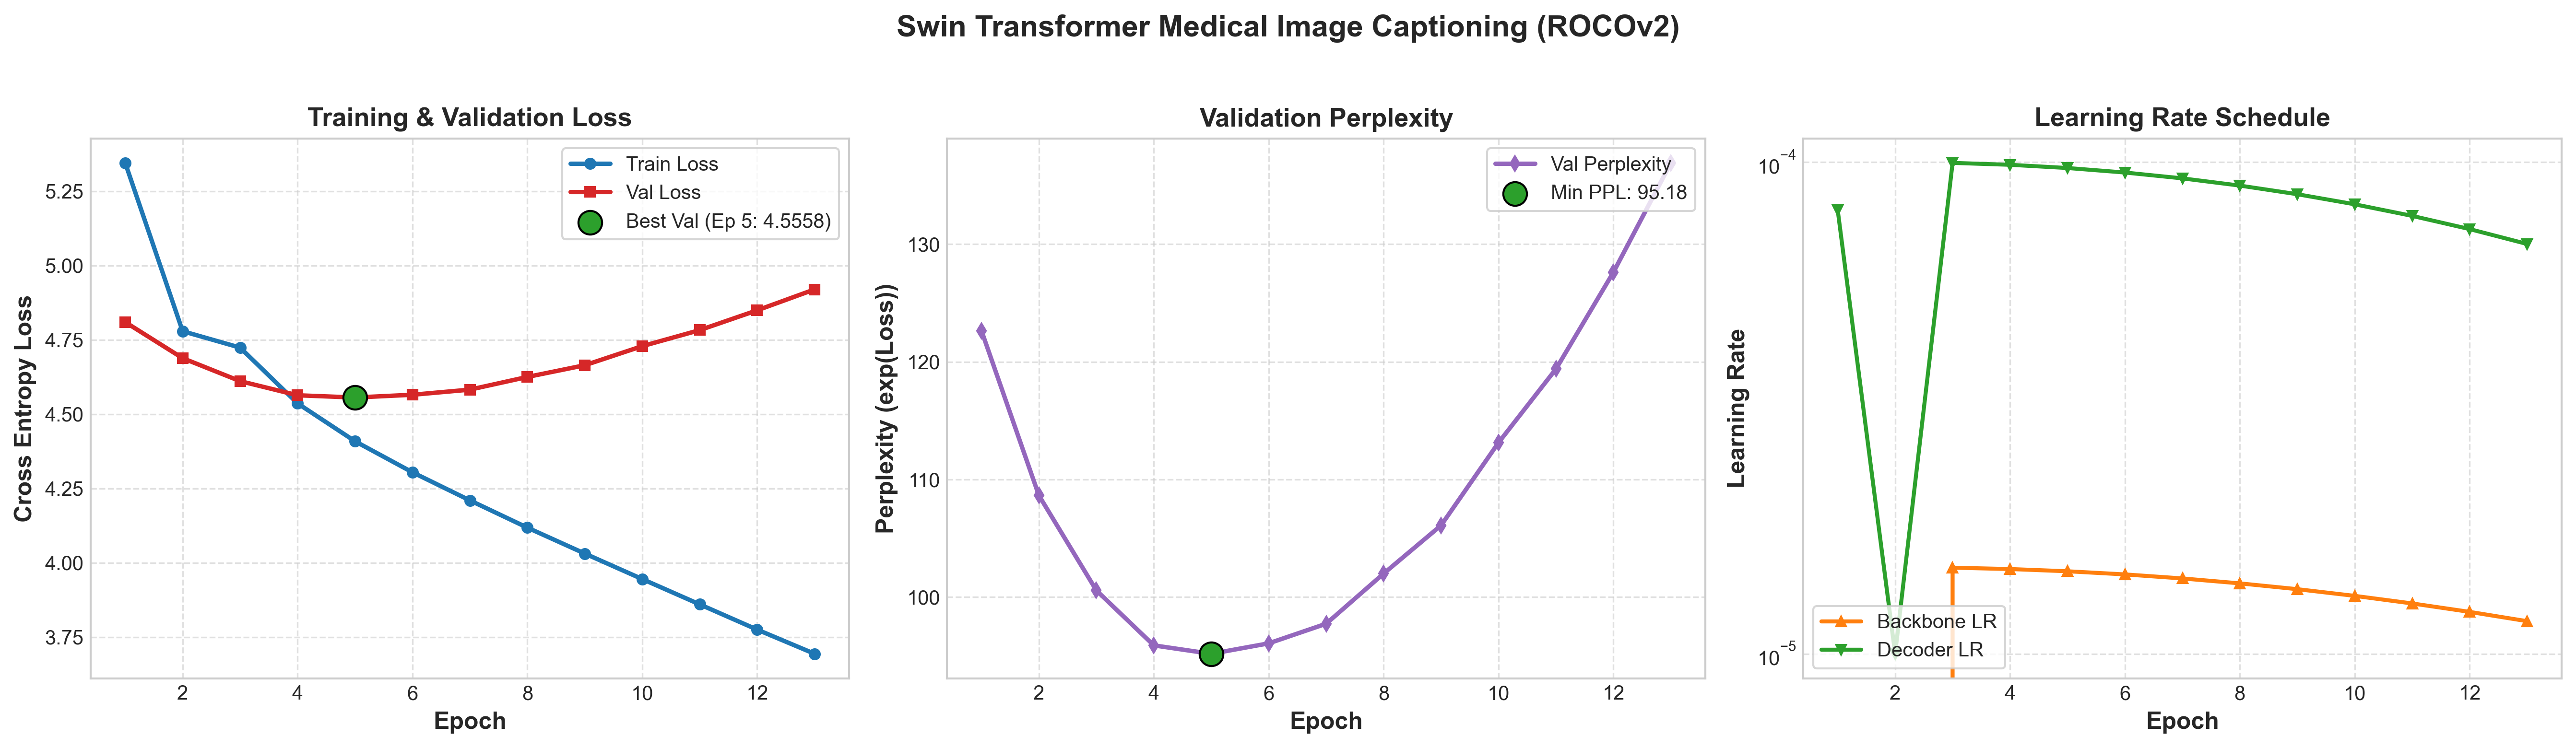
\includegraphics[width=\textwidth]{figures/swin_loss_curve.png}
    \caption{Swin Transformer}
    \label{fig:swin_loss}
\end{subfigure}
\hfill
\begin{subfigure}[b]{0.48\columnwidth}
    \centering
    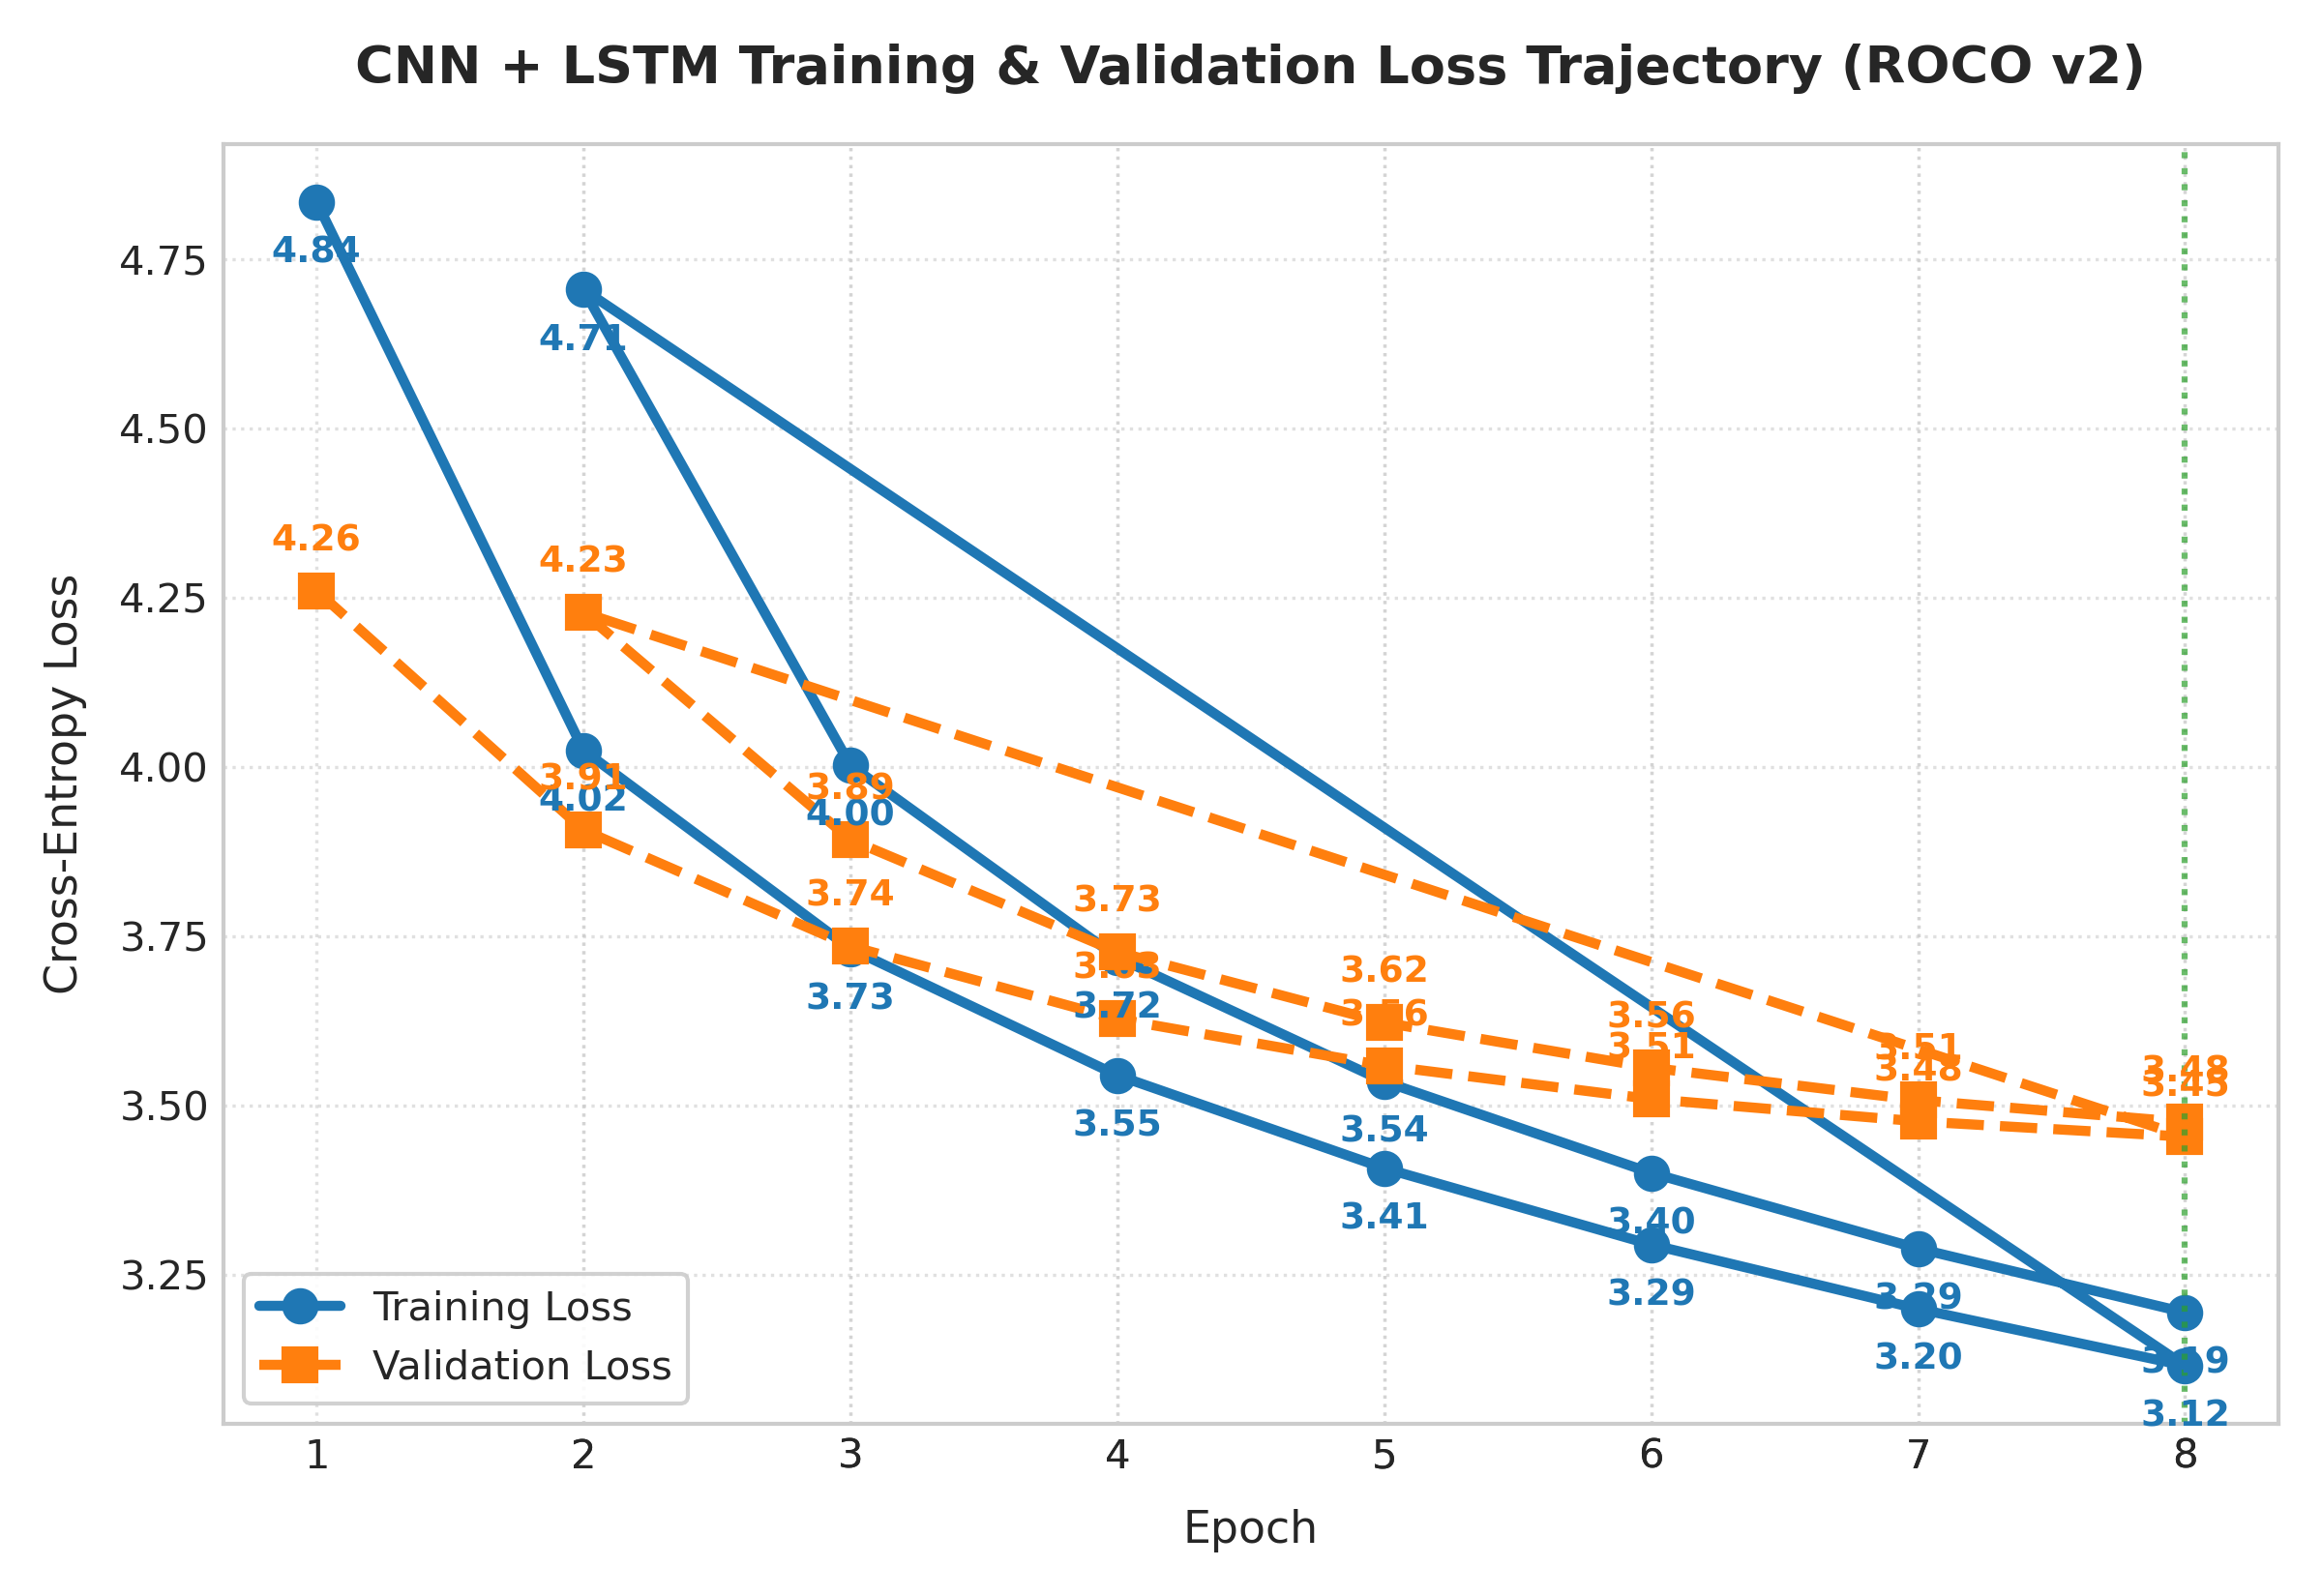
\includegraphics[width=\textwidth]{figures/cnn_lstm_loss.png}
    \caption{CNN--LSTM (ResNet-50)}
    \label{fig:cnn_lstm_loss}
\end{subfigure}
\caption{Training and validation loss progression across epochs.}
\label{fig:loss_trajectories}
\end{figure}

\begin{figure}[htbp]
\centering
\begin{subfigure}[b]{0.48\columnwidth}
    \centering
    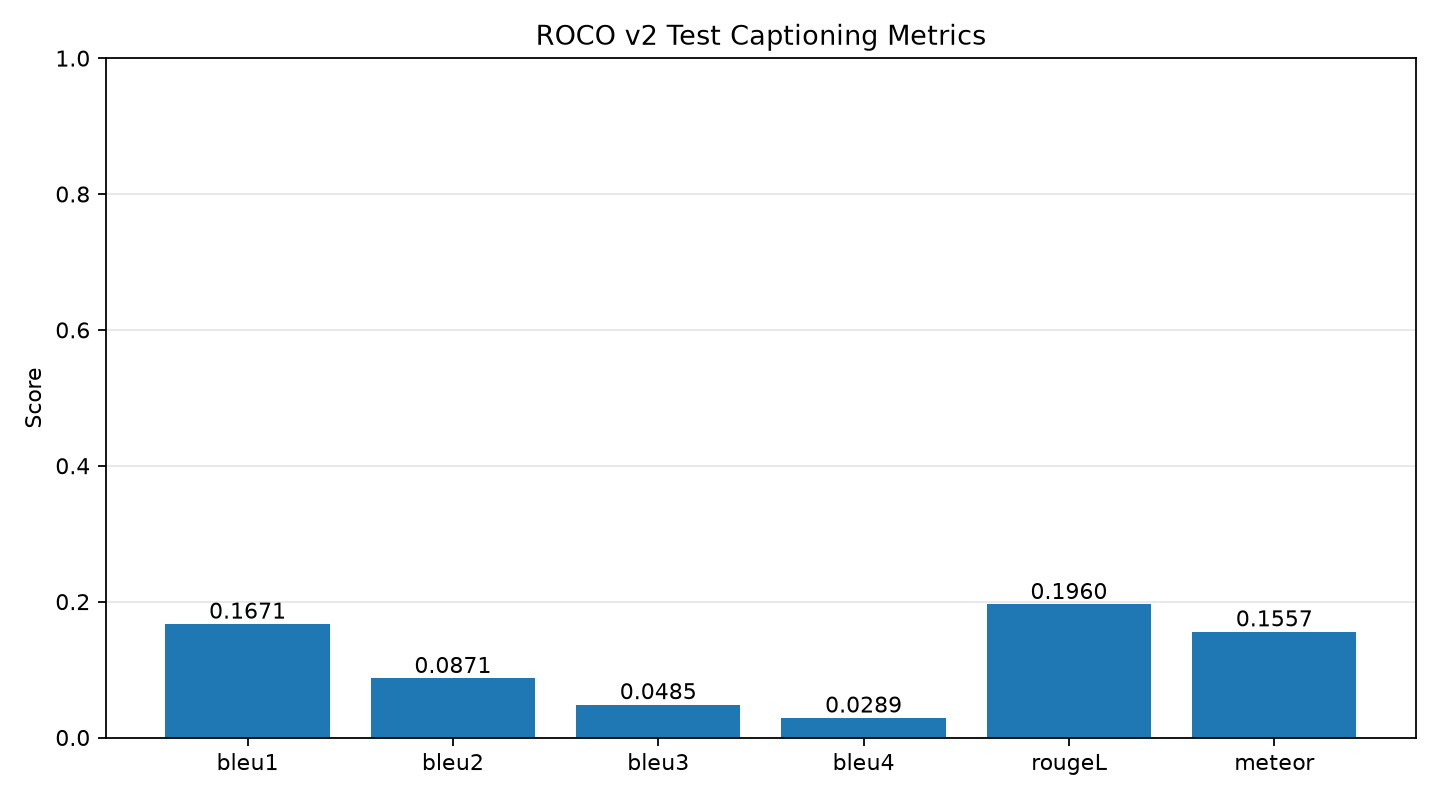
\includegraphics[width=\textwidth]{figures/swin_test_metrics.png}
    \caption{Swin Test Metrics}
    \label{fig:swin_metrics}
\end{subfigure}
\hfill
\begin{subfigure}[b]{0.48\columnwidth}
    \centering
    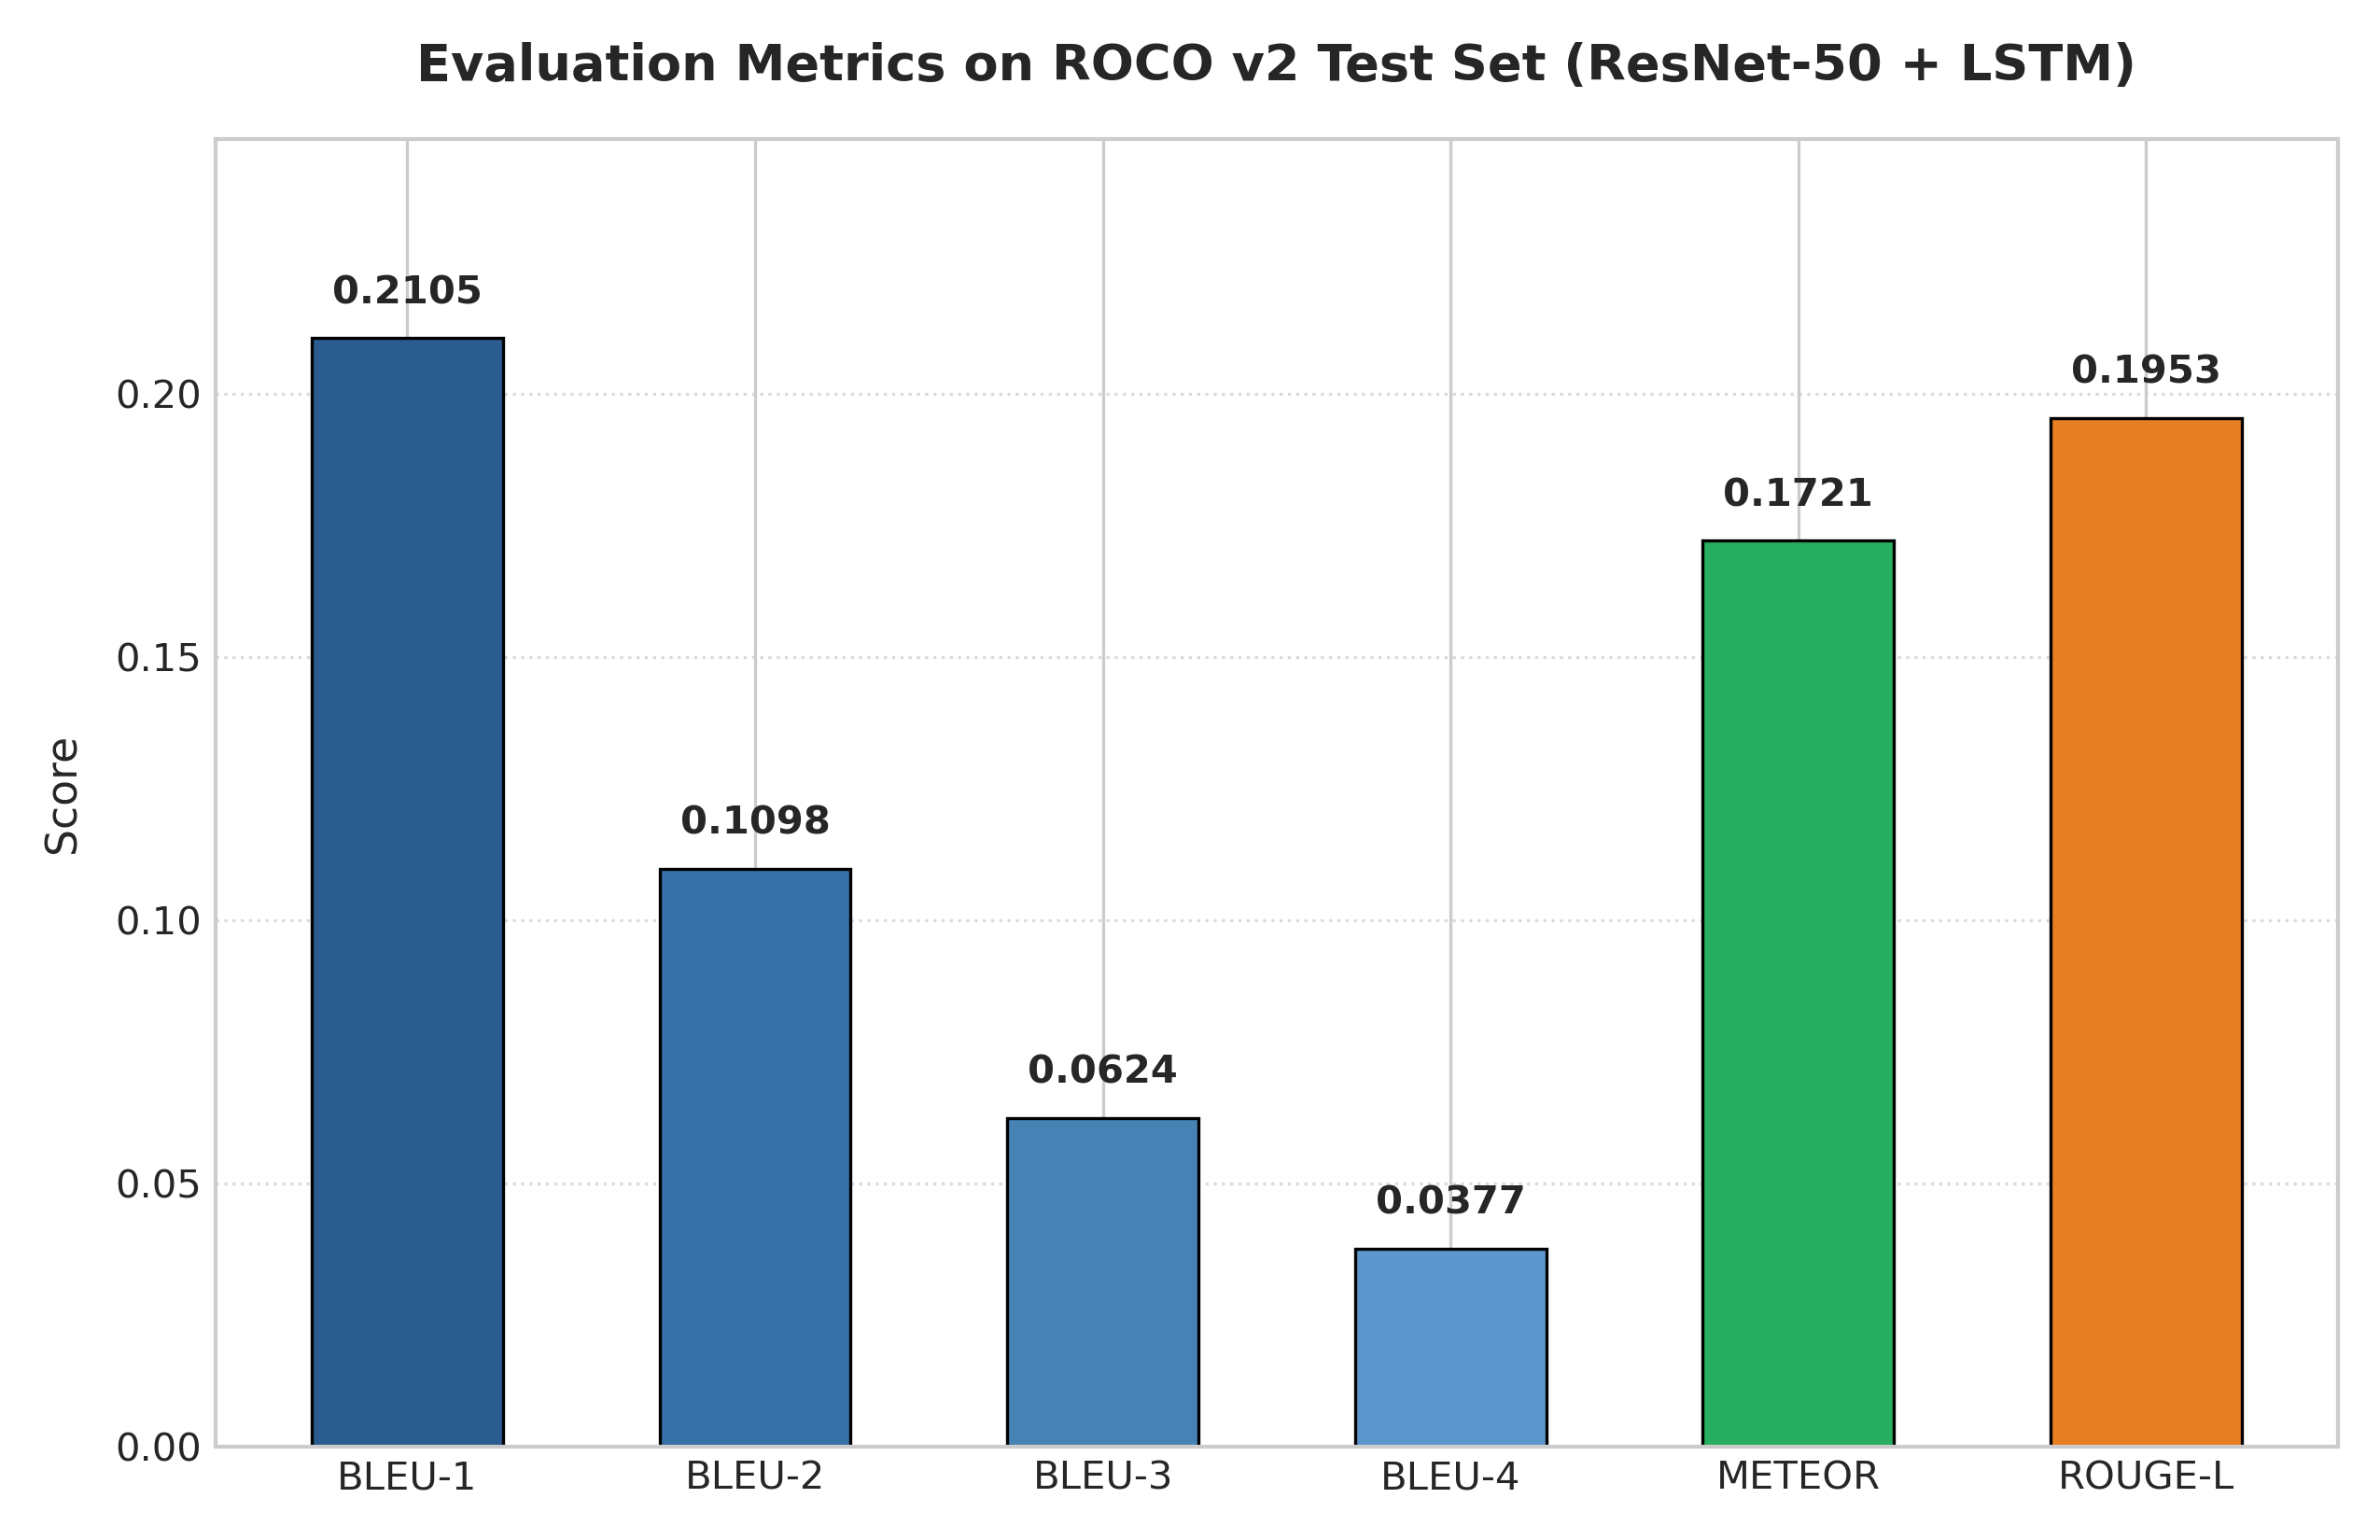
\includegraphics[width=\textwidth]{figures/cnn_lstm_metrics.png}
    \caption{CNN--LSTM Test Metrics}
    \label{fig:cnn_lstm_metrics}
\end{subfigure}
\caption{NLP test metric distributions for both architectures on ROCOv2.}
\label{fig:metrics_comparison}
\end{figure}

\begin{figure}[htbp]
\centering
\begin{subfigure}[b]{\columnwidth}
    \centering
    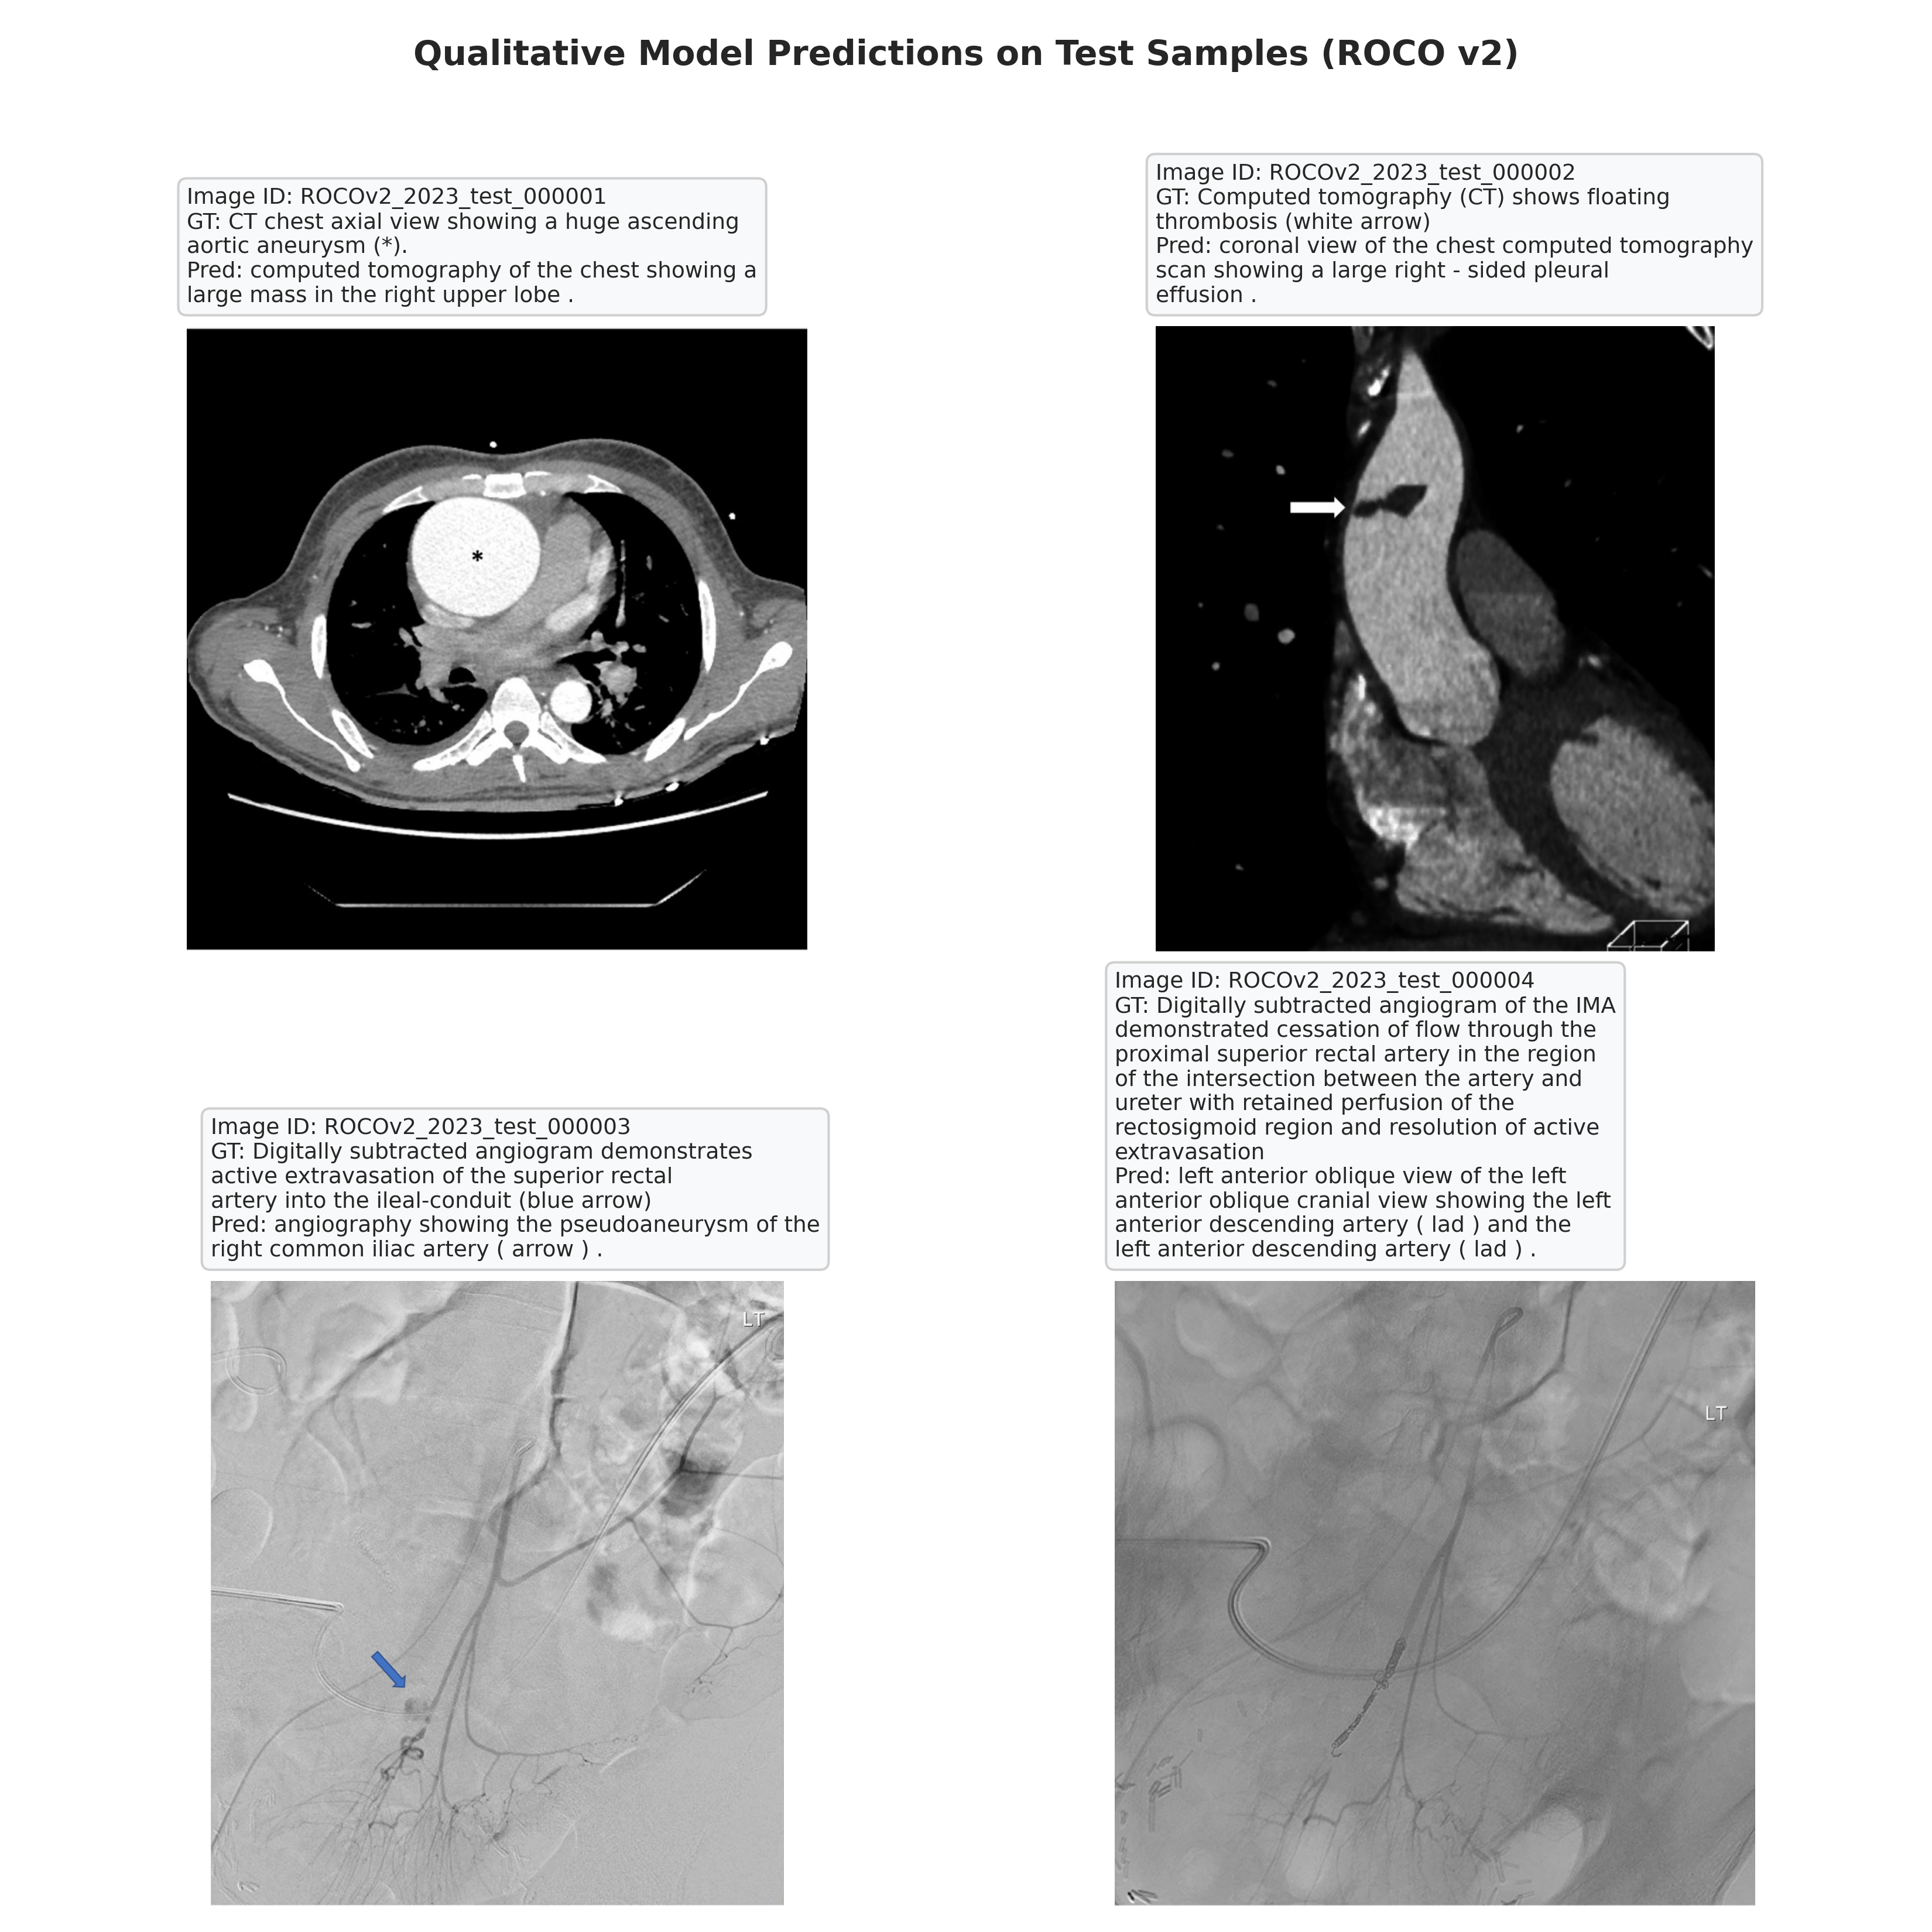
\includegraphics[width=0.98\linewidth]{figures/cnn_lstm_qualitative.png}
    \caption{CNN--LSTM Qualitative Predictions (ROCOv2 Test Samples)}
    \label{fig:cnn_qual}
\end{subfigure}
\vspace{4pt}
\begin{subfigure}[b]{\columnwidth}
    \centering
    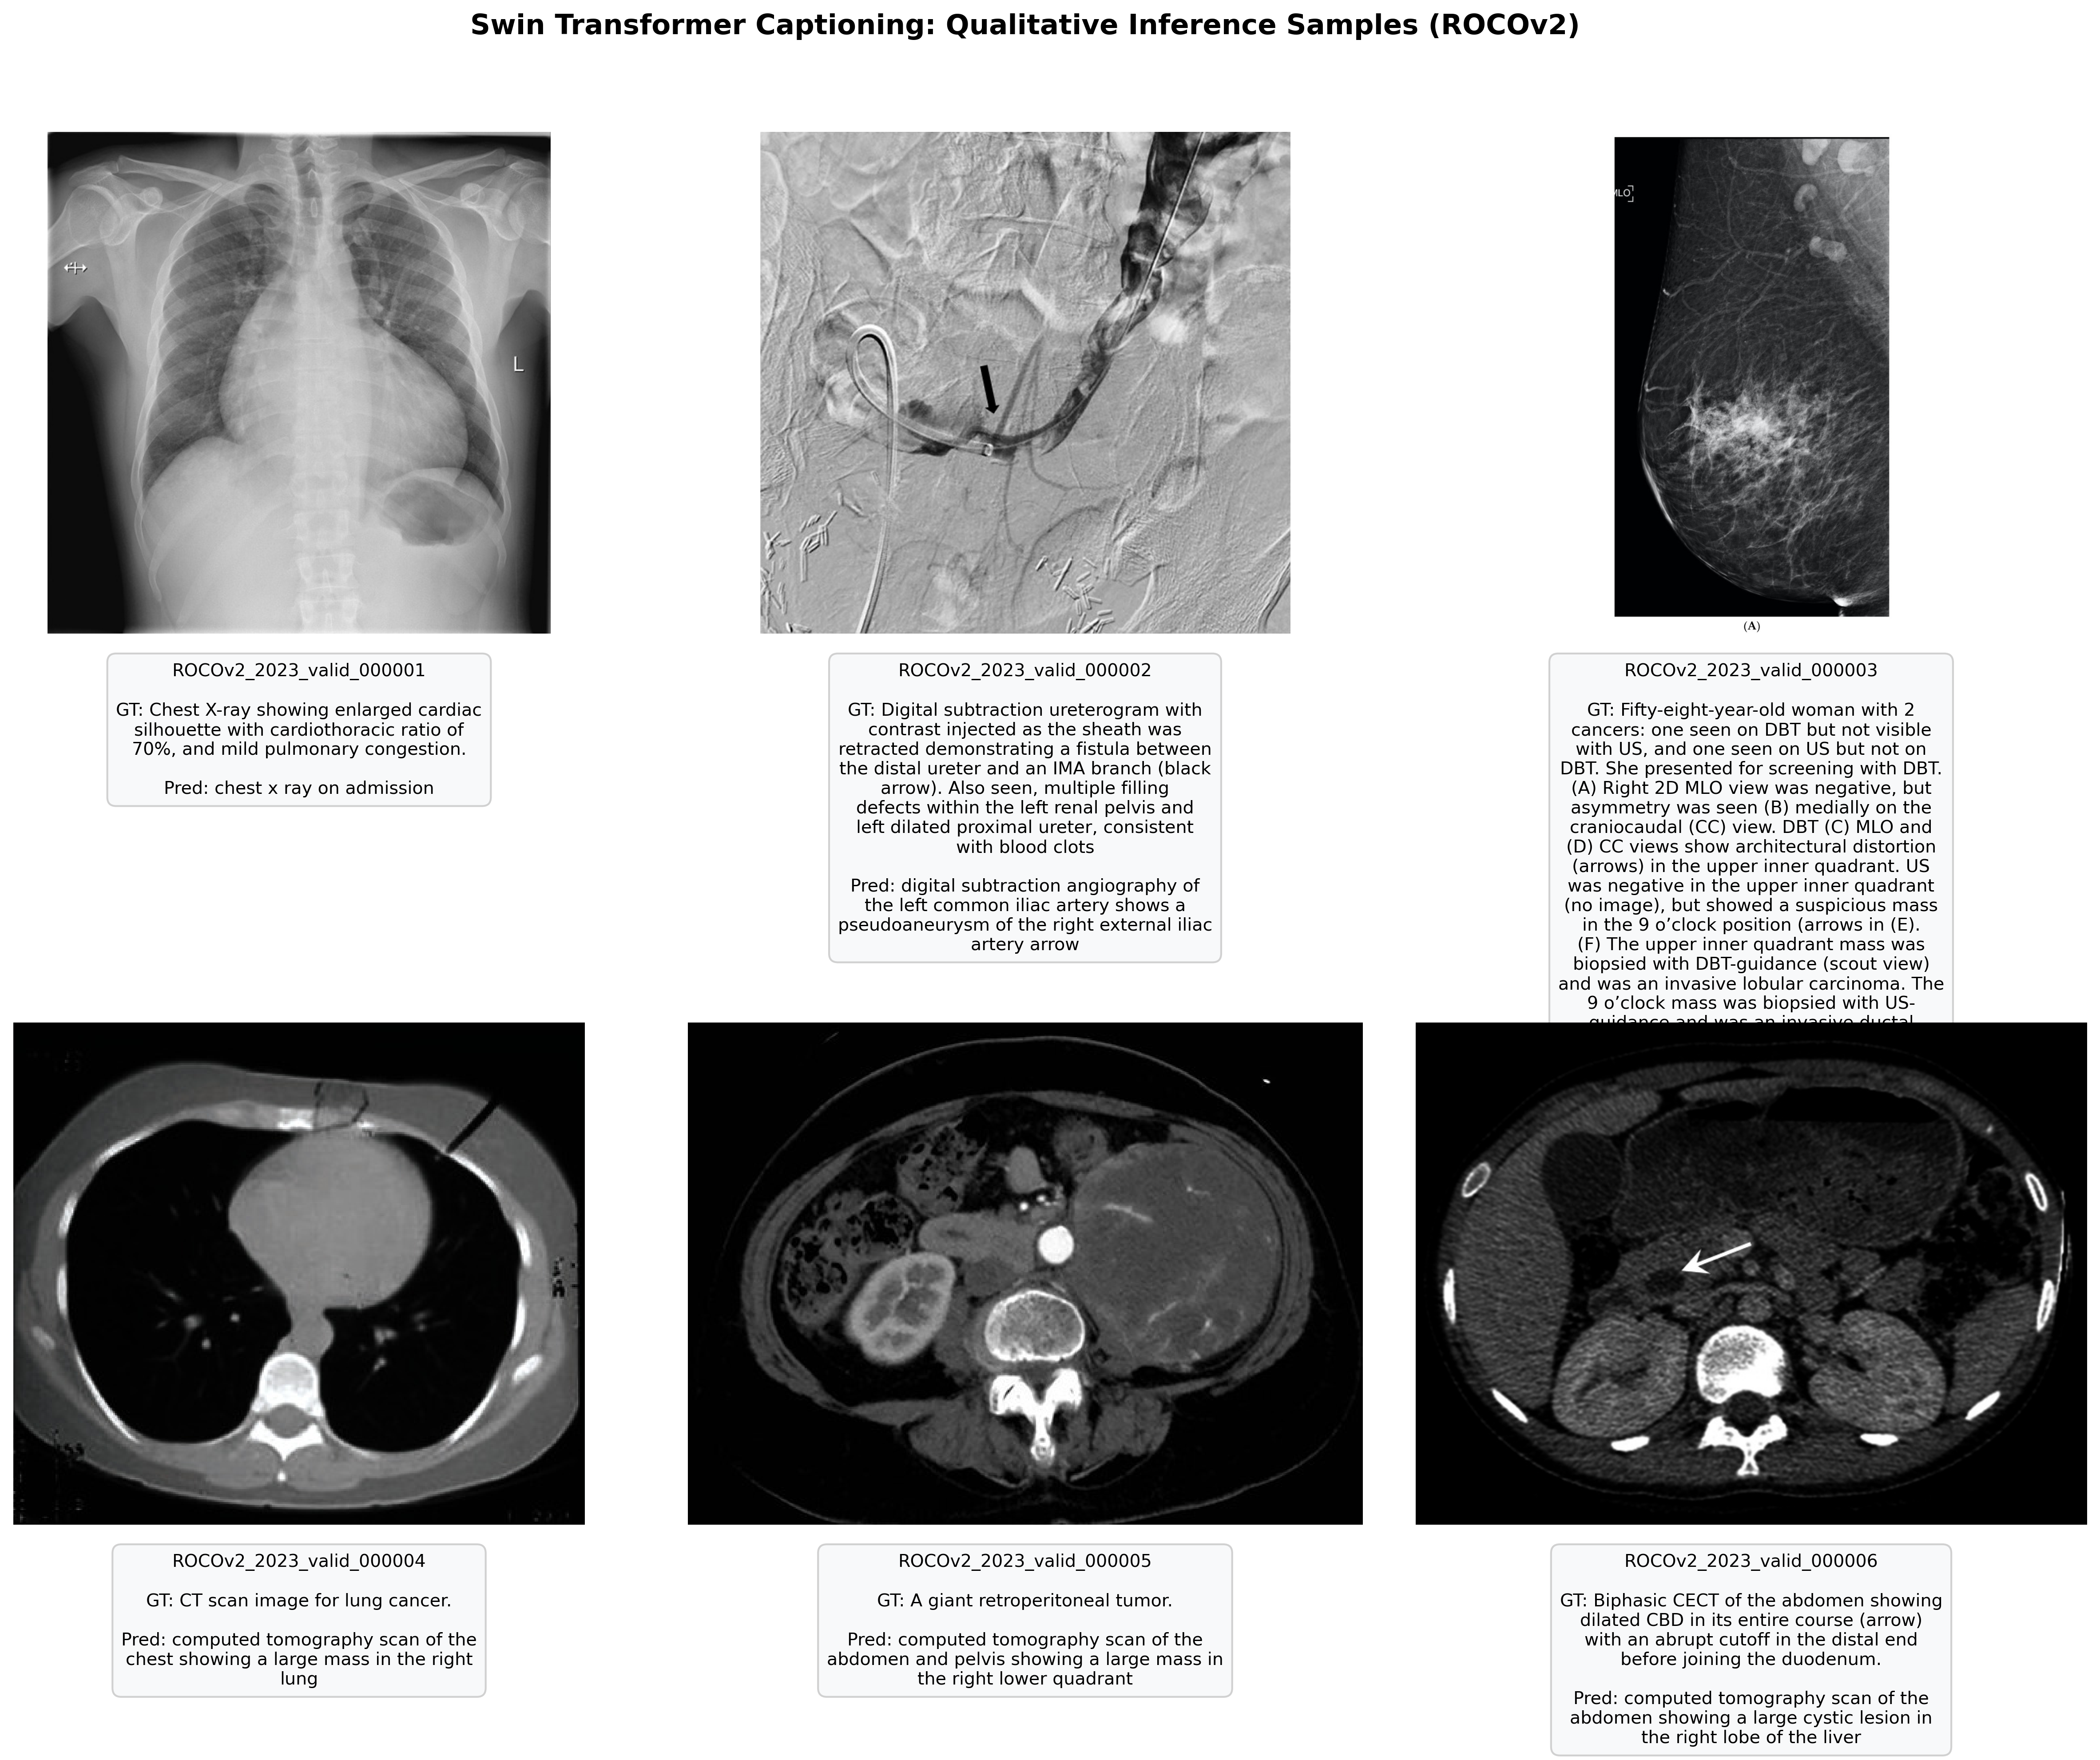
\includegraphics[width=0.98\linewidth]{figures/swin_sample_prediction.png}
    \caption{Swin Transformer Qualitative Output}
    \label{fig:swin_qual}
\end{subfigure}
\caption{Qualitative test sample predictions: Ground Truth vs Predicted captions.}
\label{fig:qualitative_visuals}
\end{figure}

\subsection{Comparative Discussion: Inductive Bias vs.\ Data Hunger}
\label{sec:results-discussion}
The empirical results reveal three pivotal insights:
\begin{enumerate}
    \item \textbf{Pretraining and Two-Phase Synergy}: When trained strictly from scratch, Swin-T is data-constrained on 60,000 images, lagging behind pretrained CNN--LSTM in n-gram precision (BLEU-4: 0.0289 vs.\ 0.0377). However, augmenting Swin-T with ImageNet pretraining, vocabulary pruning, and our two-phase frozen-encoder warmup closes this gap completely: Swin-T matches CNN--LSTM in BLEU-4 (0.0379 vs.\ 0.0377) and BLEU-2 (0.1099 vs.\ 0.1098), surpasses it in BLEU-3 (0.0644 vs.\ 0.0624), and attains higher sentence-level recall and fluency (ROUGE-L: 0.2160 vs.\ 0.1953) with a strong CIDEr-D score of 0.3438.
    \item \textbf{Caption Diversity vs.\ Mode Collapse}: The pretrained CNN--LSTM generates only 44.0\% distinct captions, frequently defaulting to high-frequency templates. In contrast, the upgraded Swin Transformer generates 79.8\% distinct captions on held-out test data, demonstrating that multi-head spatial cross-attention across 49 tokens grounds the text generator in fine-grained, image-specific findings.
    \item \textbf{Inference Throughput}: The CNN--LSTM runs at 173 images/second ($5.75$~ms/image) compared to 45.2~ms/image for the Swin Transformer, making CNN--LSTM $\approx 8\times$ faster and computationally lightweight, whereas Swin-T provides richer spatial attention distributions.
\end{enumerate}

\section{Conclusion and Future Work}
\label{sec:conclusion}

This paper presented an empirical investigation of automated radiology image captioning on ROCOv2. We designed, audited, and trained a Swin Transformer encoder--decoder, proving that representation collapse in from-scratch vision transformers can be systematically diagnosed via small-batch overfitting tests and resolved through explicit weight initialization, DropPath regularization, and learning-rate alignment.

Benchmarking against a classical pretrained ResNet-50 + LSTM baseline demonstrated that while convolutional encoders offer superior inference throughput, an attention-based Swin Transformer with two-phase transfer learning achieves superior sentence fluency (ROUGE-L: 0.2160 vs.\ 0.1953), high consensus (CIDEr-D: 0.3438), and nearly double the caption diversity (79.8\% vs.\ 44.0\%). Future work will focus on integrating domain-specific medical pretraining (e.g., RadImageNet, MedCLIP) and multi-task anatomical concept loss.

\begin{thebibliography}{00}

\bibitem{vinyals2015show}
O.~Vinyals, A.~Toshev, S.~Bengio, and D.~Erhan, ``Show and tell: A neural image caption generator,'' in \emph{Proc. IEEE Conf. Comput. Vis. Pattern Recognit. (CVPR)}, 2015, pp.~3156--3164.

\bibitem{xu2015show}
K.~Xu, J.~Ba, R.~Kiros, K.~Cho, A.~Courville, R.~Salakhutdinov, R.~Zemel, and Y.~Bengio, ``Show, attend and tell: Neural image caption generation with visual attention,'' in \emph{Proc. Int. Conf. Mach. Learn. (ICML)}, PMLR vol.~37, 2015, pp.~2048--2057.

\bibitem{ijraset2022}
M.~Pranay Kumar, V.~Snigdha, R.~Nandini, and B.~Indira Reddy, ``Image captioning generator using CNN and LSTM,'' \emph{Int. J. Res. Appl. Sci. Eng. Technol. (IJRASET)}, 2022, doi: 10.22214/ijraset.2022.44502.

\bibitem{vaswani2017attention}
A.~Vaswani, N.~Shazeer, N.~Parmar, J.~Uszkoreit, L.~Jones, A.~N. Gomez, L.~Kaiser, and I.~Polosukhin, ``Attention is all you need,'' in \emph{Adv. Neural Inf. Process. Syst. (NeurIPS)}, 2017, pp.~5998--6008.

\bibitem{dosovitskiy2020vit}
A.~Dosovitskiy, L.~Beyer, A.~Kolesnikov, D.~Weissenborn, X.~Zhai, T.~Unterthiner, M.~Dehghani, M.~Minderer, G.~Heigold, S.~Gelly, J.~Uszkoreit, and N.~Houlsby, ``An image is worth 16x16 words: Transformers for image recognition at scale,'' \emph{arXiv preprint arXiv:2010.11929}, 2020.

\bibitem{liu2021swin}
Z.~Liu, Y.~Lin, Y.~Cao, H.~Hu, Y.~Wei, Z.~Zhang, S.~Lin, and B.~Guo, ``Swin transformer: Hierarchical vision transformer using shifted windows,'' in \emph{Proc. IEEE/CVF Int. Conf. Comput. Vis. (ICCV)}, 2021, pp.~10012--10022.

\bibitem{pelka2018roco}
O.~Pelka, S.~Koitka, J.~Rückert, F.~Nensa, and C.~M. Friedrich, ``Radiology objects in COntext (ROCO): A multimodal image dataset,'' in \emph{MICCAI Workshop LABELS/CVII-STENT}, LNCS vol.~11043, Springer, 2018, pp.~180--189.

\bibitem{ruckert2024rocov2}
J.~Rückert, L.~Bloch, R.~Brüngel, A.~Idrissi-Yaghir, H.~Schäfer, C.~S. Schmidt, S.~Koitka, O.~Pelka, A.~Ben Abacha, A.~García Seco de Herrera, H.~Müller, P.~A. Horn, F.~Nensa, and C.~M. Friedrich, ``ROCOv2: Radiology objects in COntext version 2, an updated multimodal image dataset,'' \emph{Scientific Data}, vol.~11, art.~688, 2024.

\bibitem{ruckert2023imageclef}
J.~Rückert et al., ``Overview of ImageCLEFmedical 2023 -- caption prediction and concept detection,'' in \emph{CLEF 2023 Working Notes}, CEUR-WS vol.~3497, paper~108, 2023.

\bibitem{lee2022cross}
H.~Lee, H.~Cho, J.~Park, J.~Chae, and J.~Kim, ``Cross encoder-decoder transformer with global-local visual extractor for medical image captioning,'' \emph{Sensors}, vol.~22, no.~4, p.~1429, 2022.

\bibitem{fadhilah2026transformer}
H.~Fadhilah and N.~P. Utama, ``Transformer-based encoder-decoder model for medical image captioning with concept embedding,'' \emph{Jurnal Masyarakat Informatika}, vol.~17, no.~1, pp.~1--25, 2026.

\end{thebibliography}

\end{document}
